\documentclass[fleqn]{article}
\usepackage[margin=1in]{geometry}
\usepackage[nodisplayskipstretch]{setspace}
\usepackage{amsmath, nccmath, bm}
\usepackage{amssymb}
\usepackage{enumitem}
\usepackage{graphicx}
\usepackage{float}
\usepackage{listings}
\usepackage{hyperref}
\usepackage[svgnames]{xcolor}
\graphicspath{{./images}}

\hypersetup{
    colorlinks=true,
    linkcolor=black,
    filecolor=black,      
    urlcolor=blue
    }

\newcommand{\zerodisplayskip}{
	\setlength{\abovedisplayskip}{0pt}%
	\setlength{\belowdisplayskip}{0pt}%
	\setlength{\abovedisplayshortskip}{0pt}%
	\setlength{\belowdisplayshortskip}{0pt}%
	\setlength{\mathindent}{0pt}}
	
\definecolor{vgreen}{RGB}{104,180,104}
\definecolor{vblue}{RGB}{49,49,255}
\definecolor{vorange}{RGB}{255,143,102}

\lstdefinestyle{verilog-style}
{
    language=Verilog,
    basicstyle=\small\ttfamily,
    keywordstyle=\color{vblue},
    identifierstyle=\color{black},
    commentstyle=\color{vgreen},
    numbers=left,
    numberstyle=\tiny\color{black},
    numbersep=10pt,
    tabsize=8,
    moredelim=*[s][\colorIndex]{[}{]},
    literate=*{:}{:}1
}

\lstset{style={verilog-style},showstringspaces=false}

\makeatletter
\newcommand*\@lbracket{[}
\newcommand*\@rbracket{]}
\newcommand*\@colon{:}
\newcommand*\colorIndex{%
    \edef\@temp{\the\lst@token}%
    \ifx\@temp\@lbracket \color{black}%
    \else\ifx\@temp\@rbracket \color{black}%
    \else\ifx\@temp\@colon \color{black}%
    \else \color{vorange}%
    \fi\fi\fi
}
\makeatother

\newcommand{\code}[1]{%
	\colorbox{Gainsboro}{\texttt{#1}}%
}
		 
%\newcommand{\code}[1]{
%	\colorbox{Gainsboro}{\lstinline{#1}}
%}

\title{Homework 1}
\author{Owen Sowatzke}
\date{February 9, 2025}

\begin{document}

	\offinterlineskip
	\setlength{\lineskip}{12pt}
	\zerodisplayskip
	\maketitle
	
	\begin{enumerate}
		\item Given below is an illustrative layout of an inverter. Write down the material layer used according to color and arrange them in the order of fabrication.
		
		\begin{figure}[H]				
			\centerline{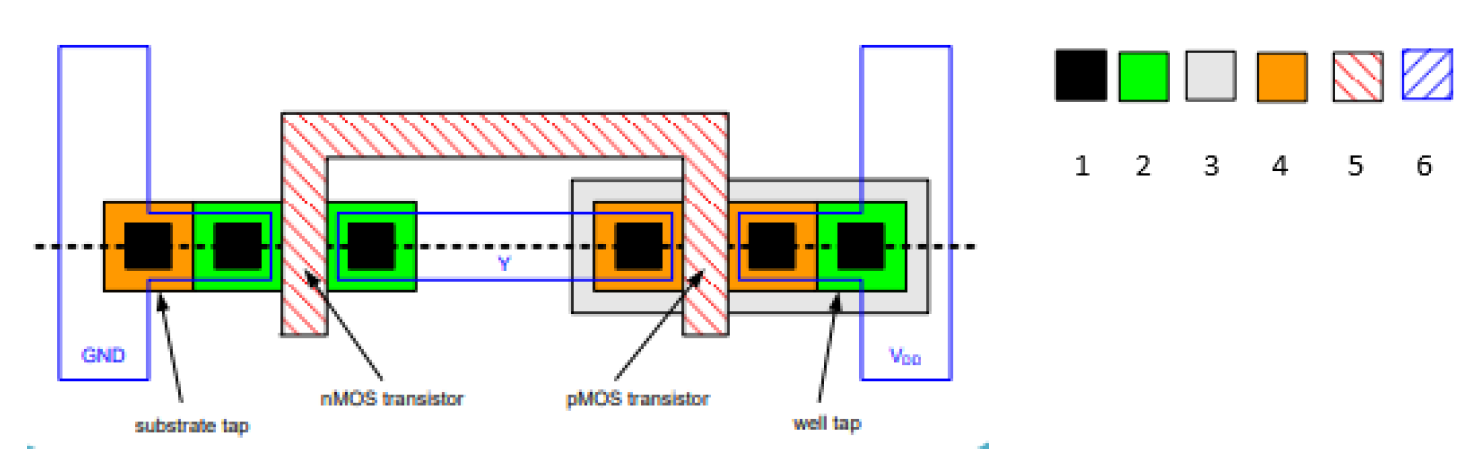
\includegraphics[width=0.8\textwidth]{inverter_layout.png}}
			\label{fig::inverter_layout}
		\end{figure}
		
		The materials in the layout are defined as follows:
		
		\begin{itemize}
			\item Material 1 (solid black) is contact material. It is made of metal (usually aluminum).
			\item Material 2 (solid green) is n+ diffusion (heavily doped n-type semiconductor [usually Si])
			\item Material 3 (solid gray) is the n-well (lightly doped n-type semiconductor [usually Si])
			\item Material 4 (solid orange) is the p+ diffusion (heavily doped p-type semiconductor [usually Si])
			\item Material 5 (striped red) is the polysilicon.
			\item Material 6 (striped blue) is the metal1 (usually aluminum)
		\end{itemize}
		
		The material layers are fabricated from the bottom up in the following order:
		
		\begin{enumerate}
			\item[1.] Material 3 (the n-well)
			\item[2.] Material 5 (polysilicon)
			\item[3.] Material 2 (n+ diffusion)
			\item[4.] Material 3 (p+ diffusion)
			\item[5.] Material 1 (contact)
			\item[6.] Material 6 (metal1)
		\end{enumerate}
		
		\item Illustrate the CMOS Layout and Stick diagram for the following Boolean expressions.
		
		\begin{enumerate}
			\item $Y = (A+B)\cdot(C+D)$
			
			In CMOS circuit design, we implement circuits that are the complement of boolean expressions. Because the provided expression is not in complement form, we must design a circuit to get $\bar{Y}$ and append an inverter to get $Y$.
			
			We start by designing the pull-down circuit to get $\bar{Y}$. We replace each ``or" with a parallel set of nmos gates and each ``and" with a series of nmos gates. The pull-down circuit is shown in the bottom left corner of Figure \ref{fig::cmos_layout_problem_2a}. We can then use the rule of conduction complements to design the pull-up circuit. To do so, we replace each parallel set of nmos gates with a series of pmos gates and each series of nmos gates with a parallel set of pmos gates. The resulting pull-up circuit is shown in the upper left of Figure \ref{fig::cmos_layout_problem_2a}. The output $\bar{Y}$ is then fed into an inverter to get $Y$.
			
			\begin{figure}[H]
				\centerline{\fbox{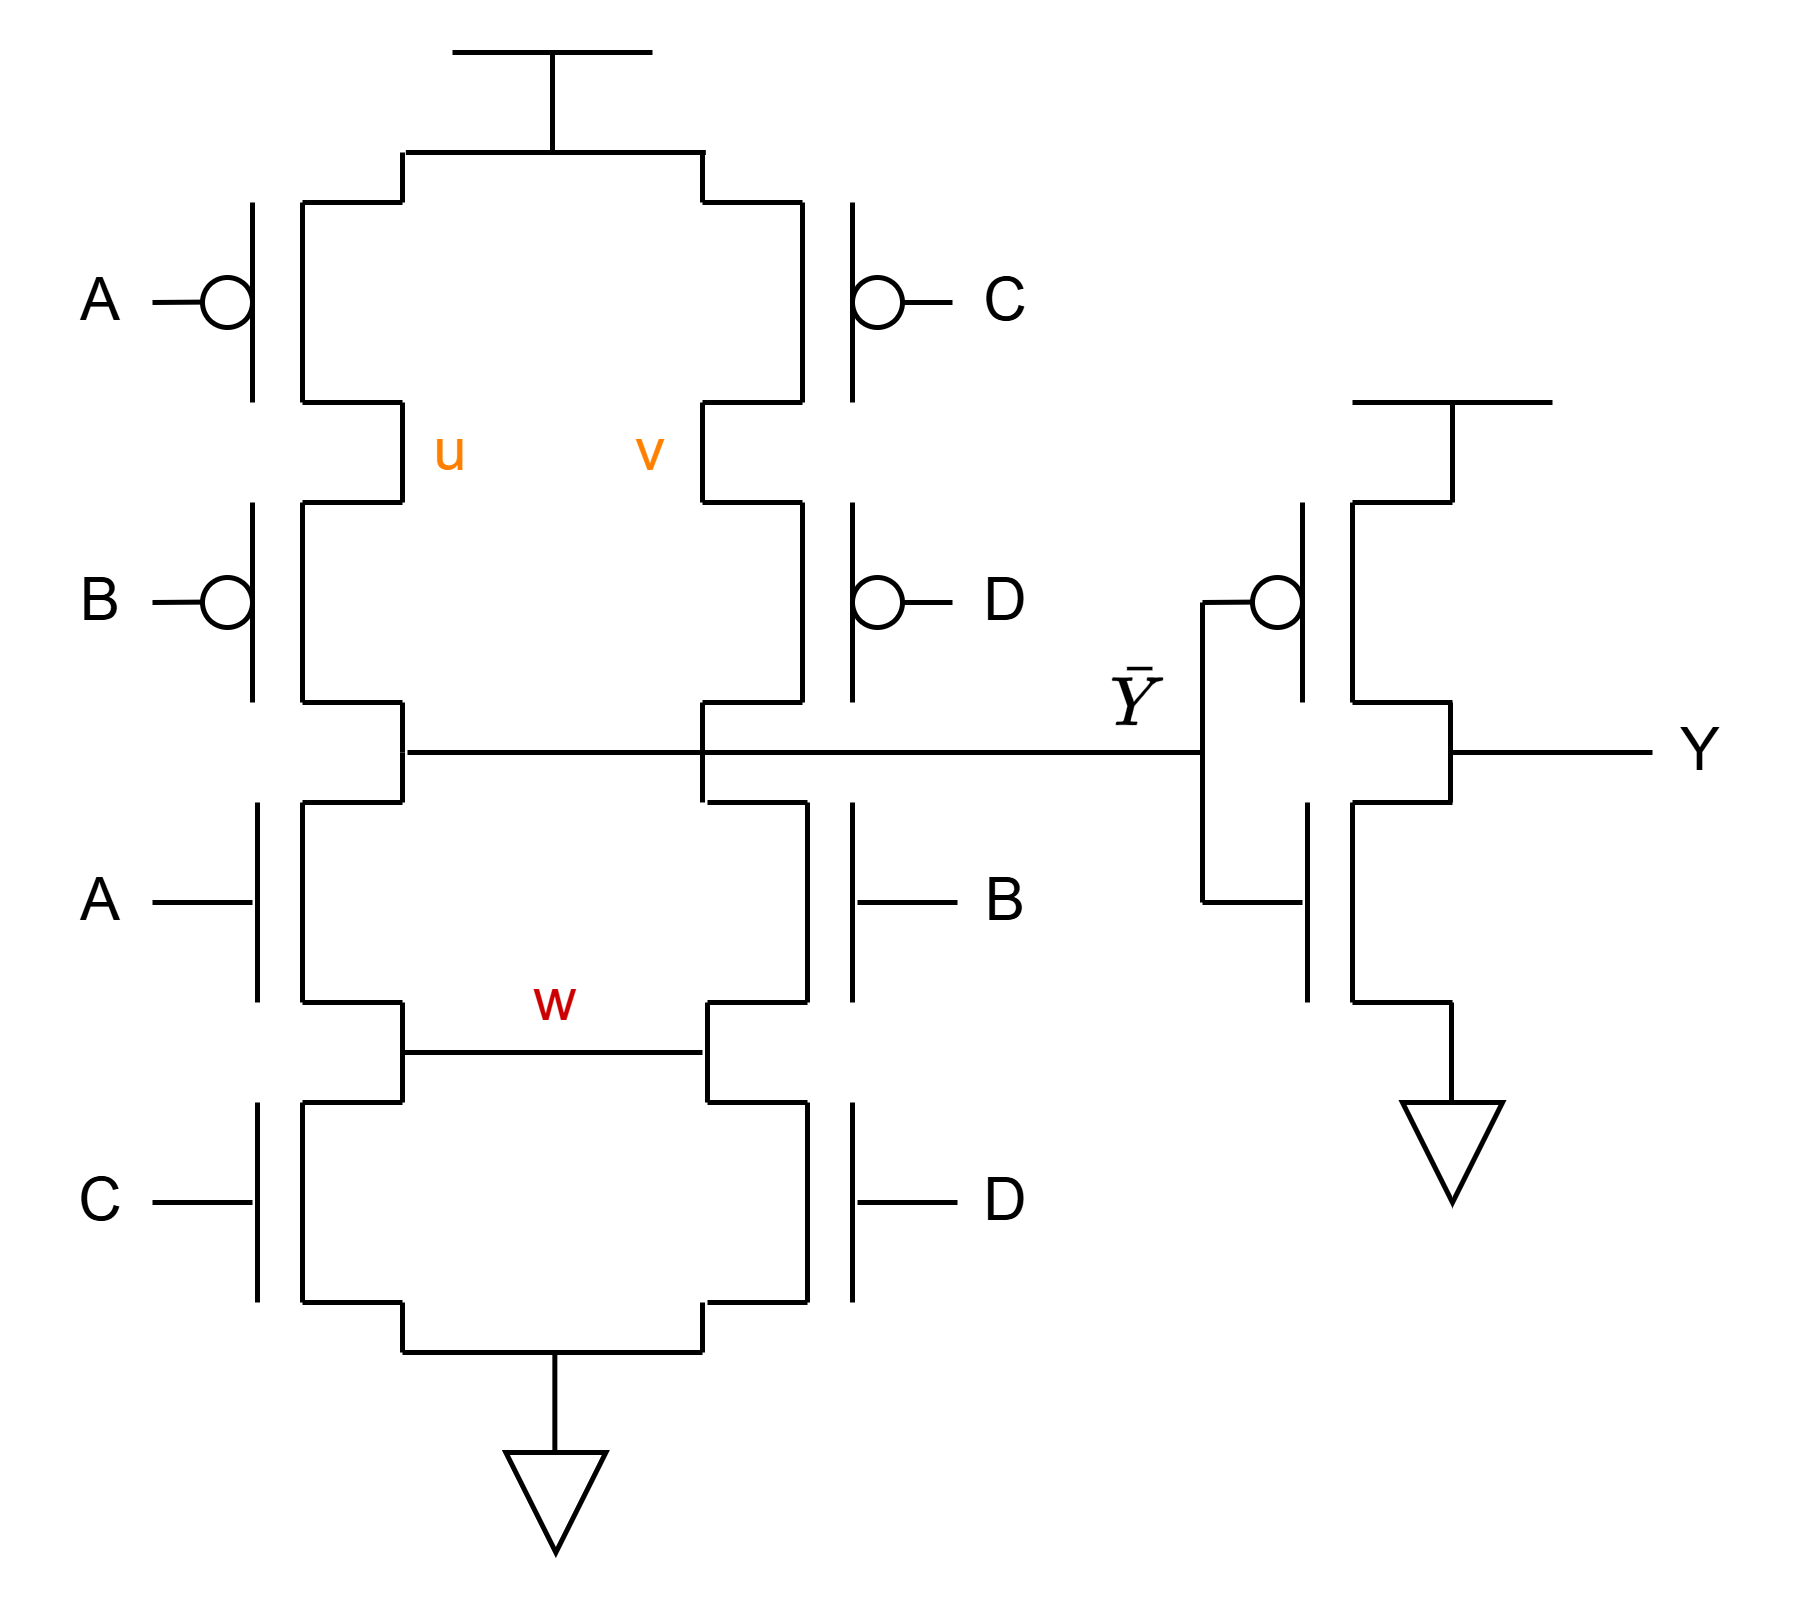
\includegraphics[width=0.5\textwidth]{cmos_layout_problem_2a.png}}}
				\caption{CMOS Layout for Problem 2a}
				\label{fig::cmos_layout_problem_2a}
			\end{figure}
			
			Because we know how to design an inverter, we consider only the circuit which generates $\bar{Y}$. To determine the order of the stick diagram inputs, we must find a Euler Path through the circuit. The Euler Path for this circuit has been traced out in the logic diagram shown in Figure \ref{fig::logic_diagram_problem_2a}.
			
			\begin{figure}[H]
				\centerline{\fbox{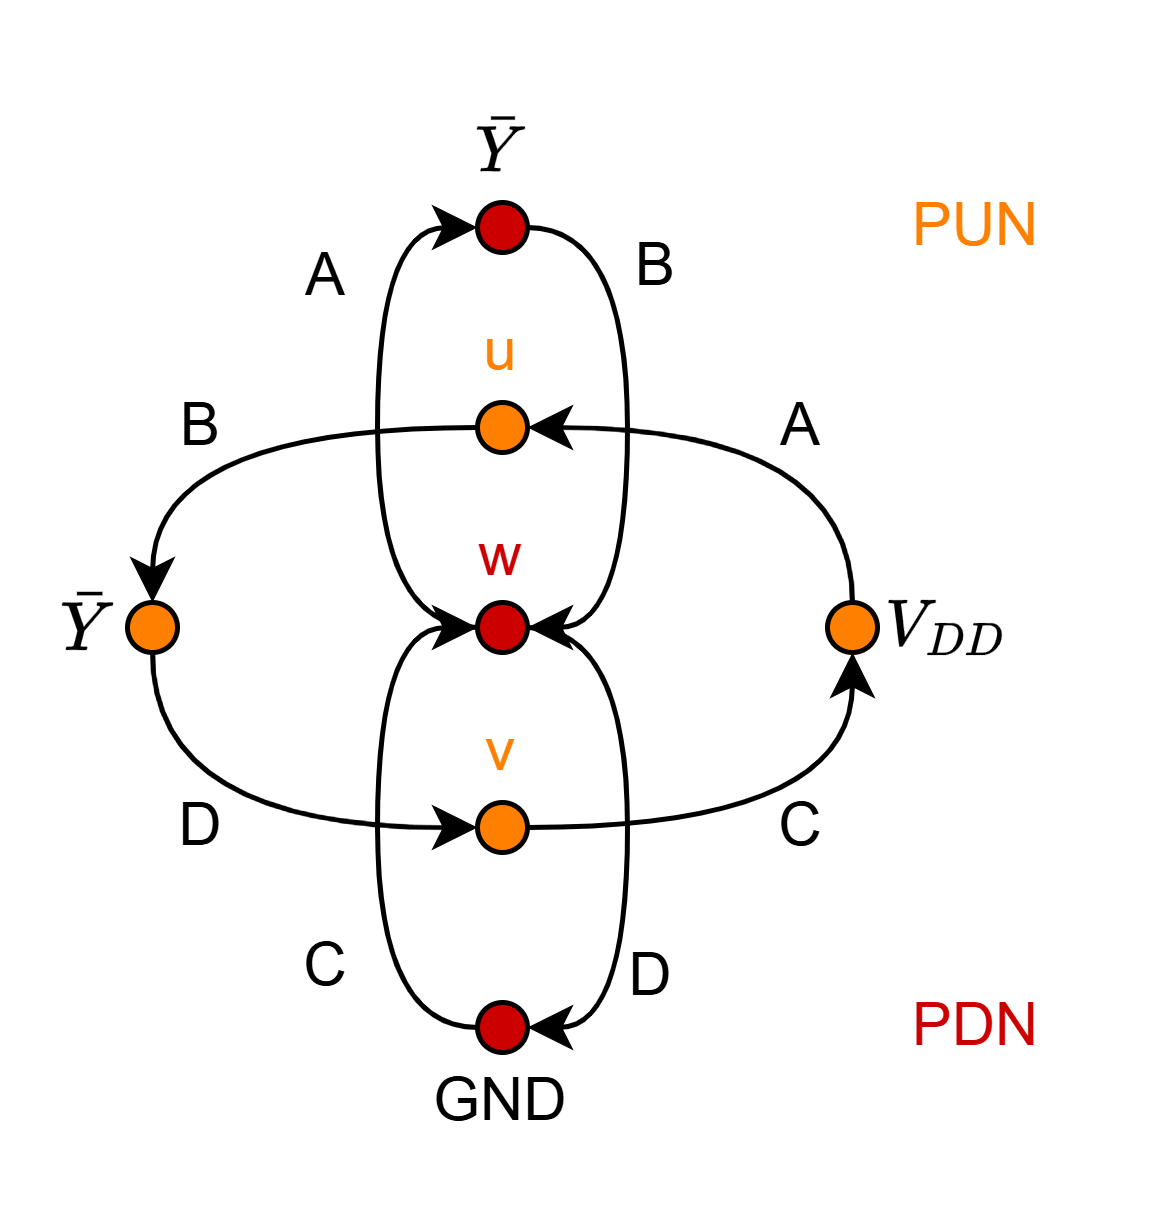
\includegraphics[width=0.4\textwidth]{logic_diagram_problem_2a.png}}}
				\caption{Logic Diagram for Problem 2a Illustrating Euler Path}
				\label{fig::logic_diagram_problem_2a}
			\end{figure}
			
			The Euler path can be found by independently tracing through all the nodes of the pull-down and pull-up networks once and only once. The path we find must also be consistent between the pull-up and pull-down networks. For this example, we determine the following input ordering: A, B, D, and C. The input ordering we find using the Euler path helps us generate a layout without diffusion breaks. Using the requested input ordering, we come up with the stick diagram shown in Figure \ref{fig::stick_diagram_problem_2a}. Note that we have also added an inverter to get $Y$ instead of $\bar{Y}$
			
			\begin{figure}[H]
				\centerline{\fbox{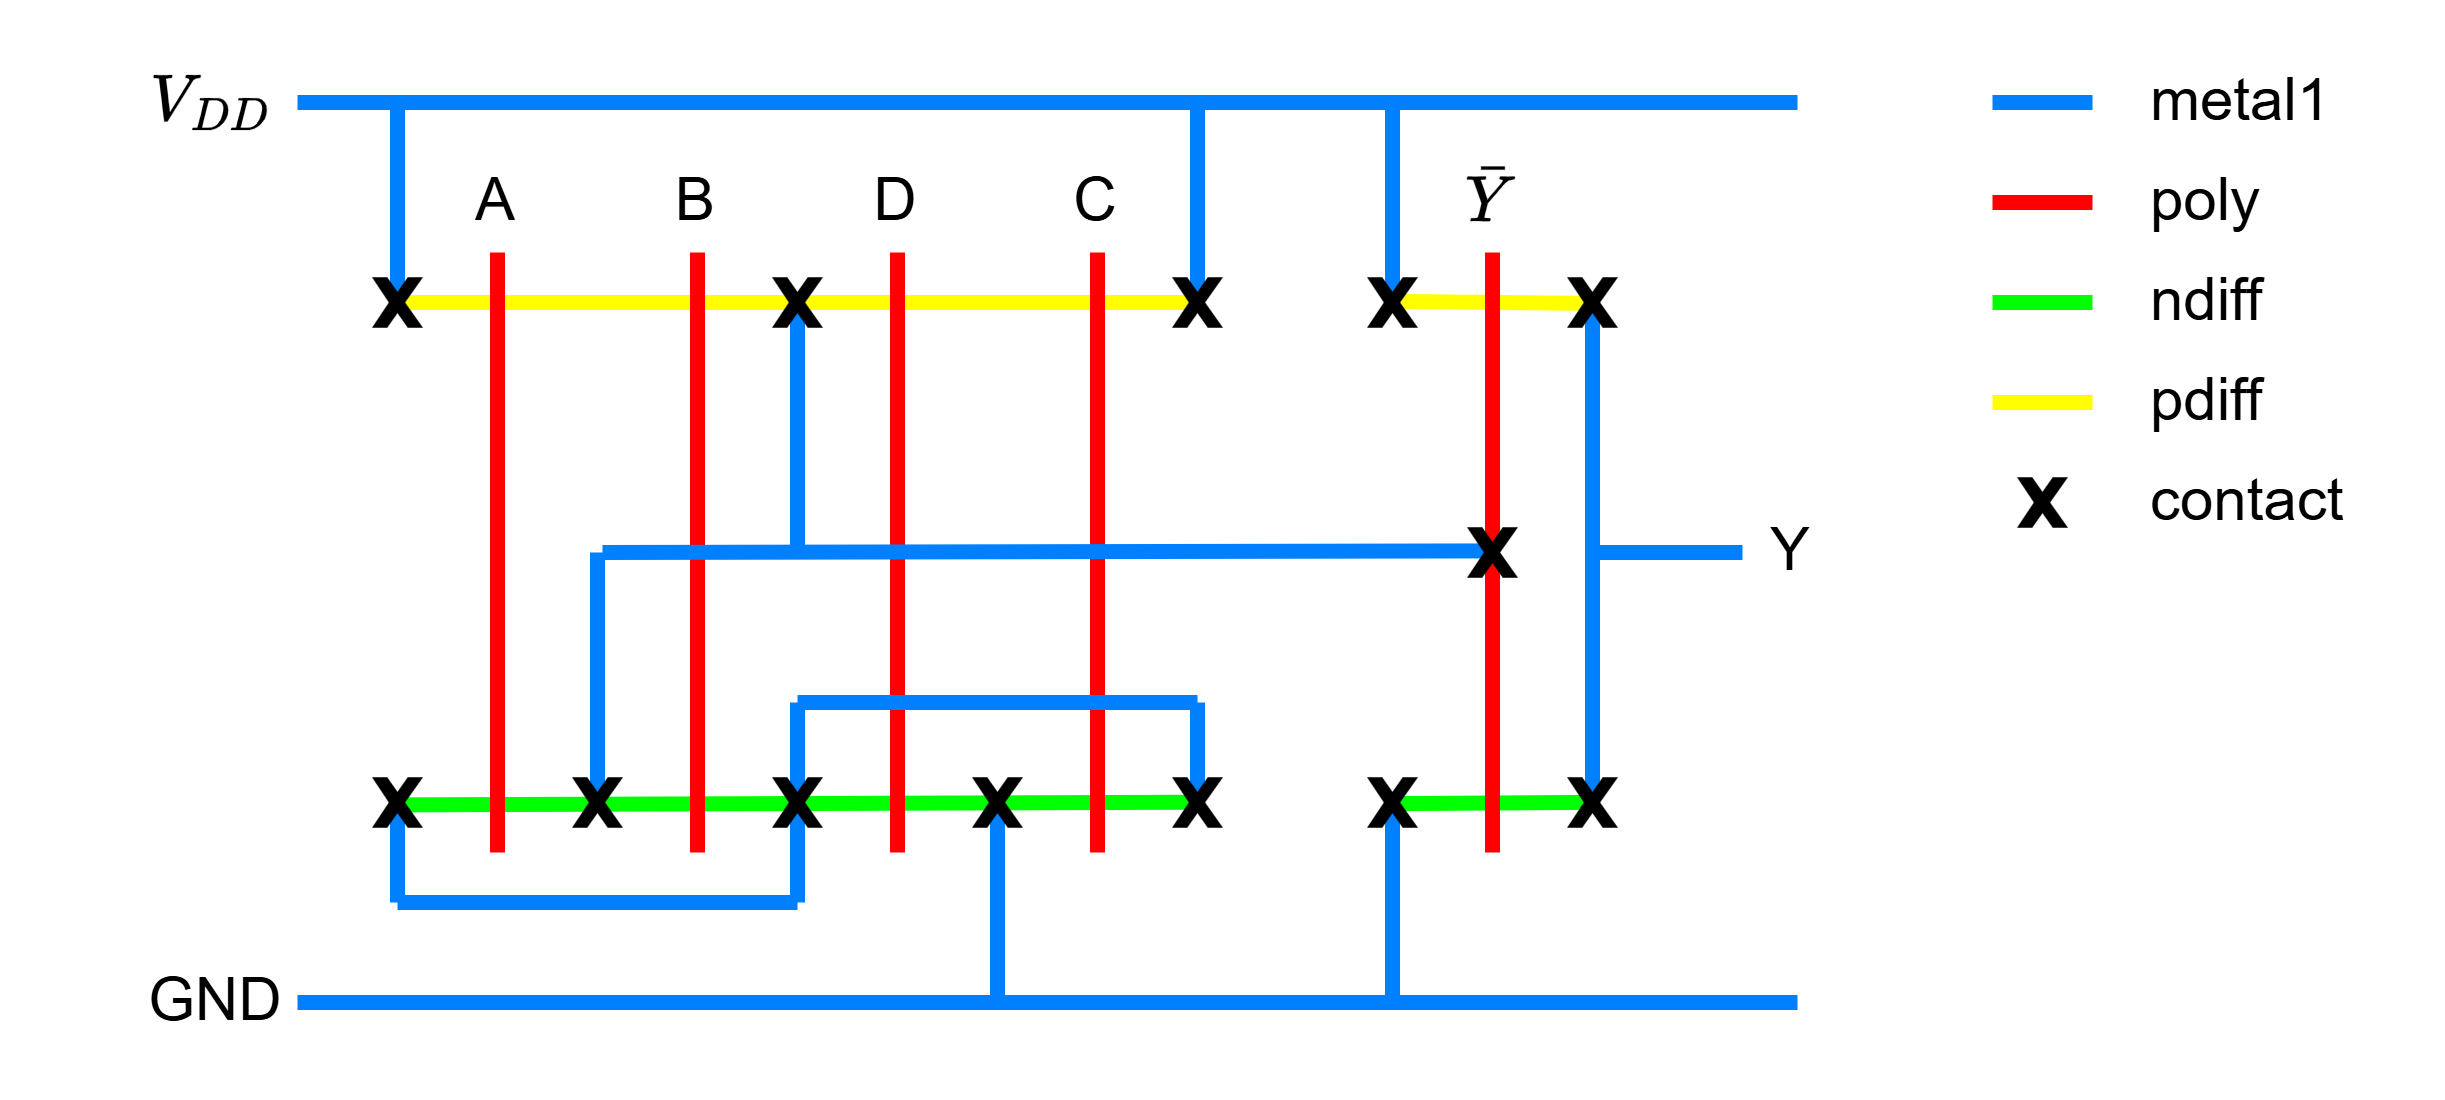
\includegraphics[width=0.6\textwidth]{stick_diagram_problem_2a.png}}}
				\caption{Stick Diagram for Problem 2a}
				\label{fig::stick_diagram_problem_2a}
			\end{figure}
			
			\item $Y = \overline{A \cdot B + C \cdot D}$
			
			The provided boolean expression is now in complemented form, so no inverter is needed. Following the steps in part a), we design the pull-down circuit for this part of the problem. The resulting pull-down circuit is shown in the bottom half of Figure \ref{fig::cmos_layout_problem_2b}. Using the rule of conduction complements, we then design the required pull-up circuit, which is shown in the top half of Figure \ref{fig::cmos_layout_problem_2b}.
			
			\begin{figure}[H]
				\centerline{\fbox{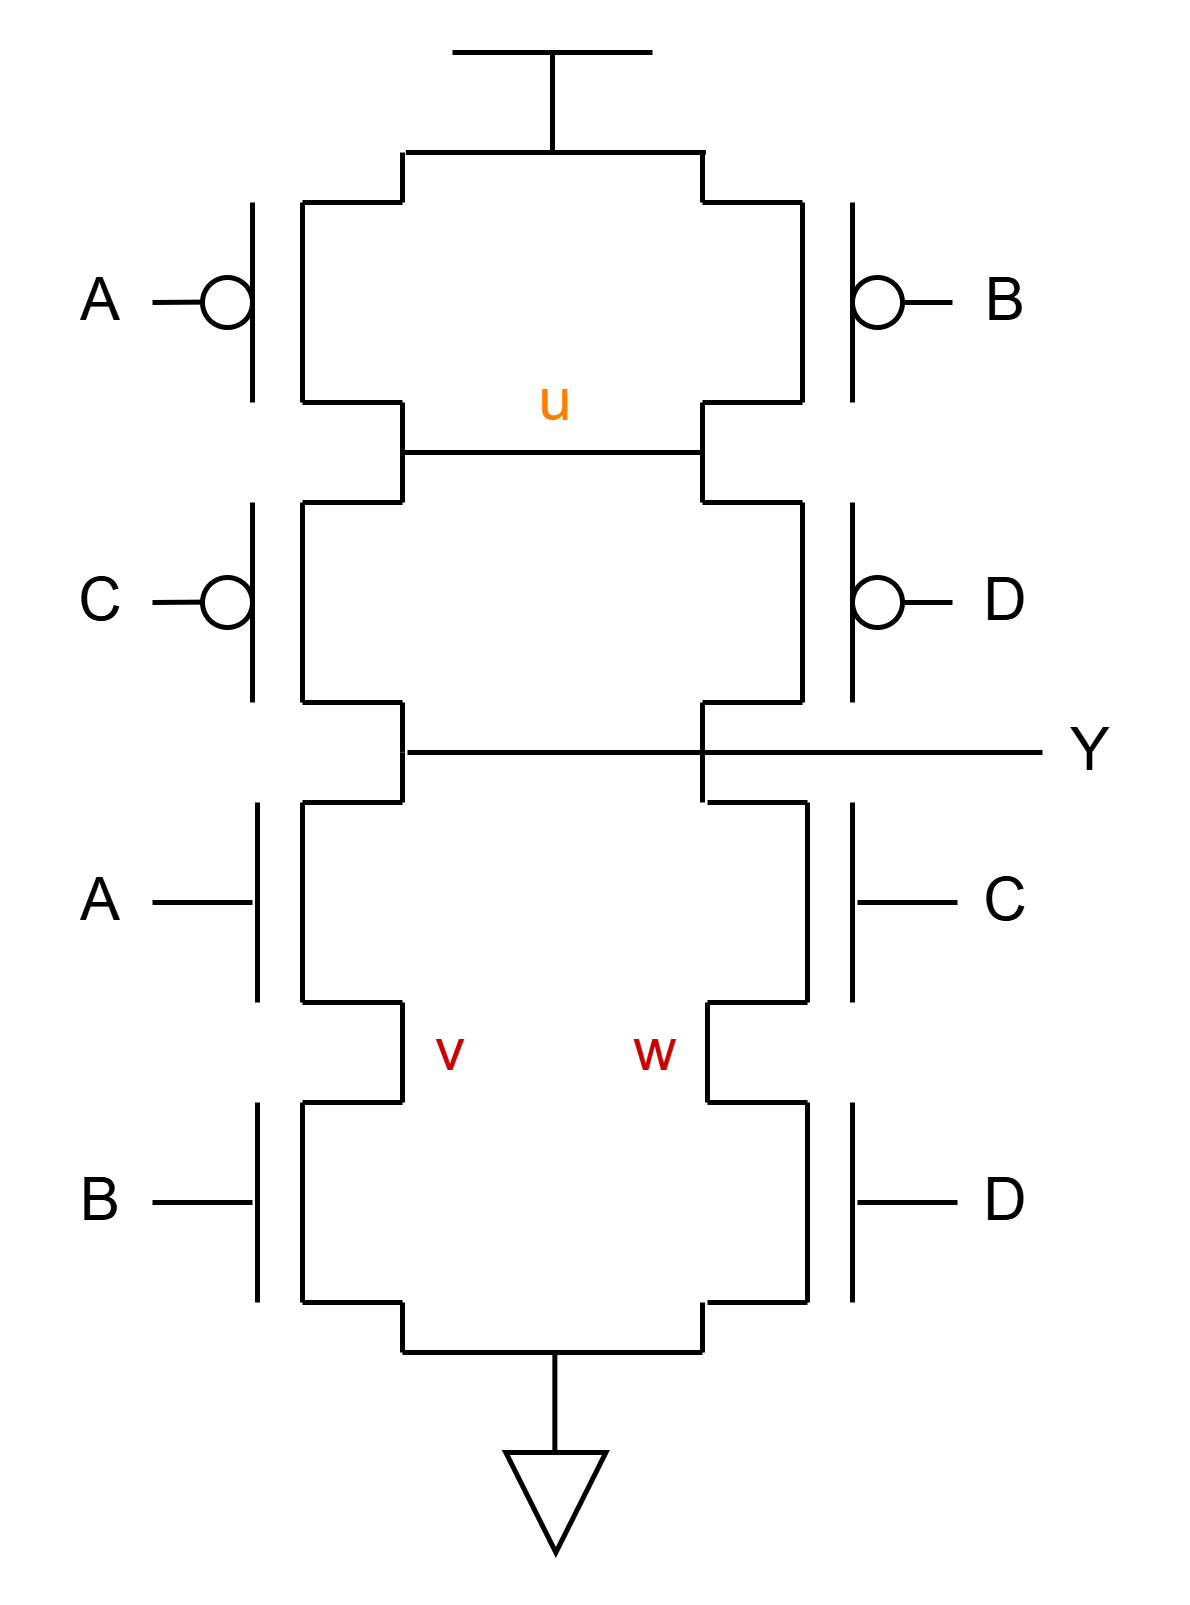
\includegraphics[width=0.35\textwidth]{cmos_layout_problem_2b.png}}}
				\caption{CMOS Layout for Problem 2b}
				\label{fig::cmos_layout_problem_2b}
			\end{figure}
			
			Next, we determine the ordering of the stick diagram inputs by find the Euler Path through the circuit. This path is illustrated in the logic diagram shown in Figure \ref{fig::logic_diagram_problem_2b}. Using the logic diagram, we find an input ordering of A, B, D, and C, identical to what was found in part a).
			
			\begin{figure}[H]
				\centerline{\fbox{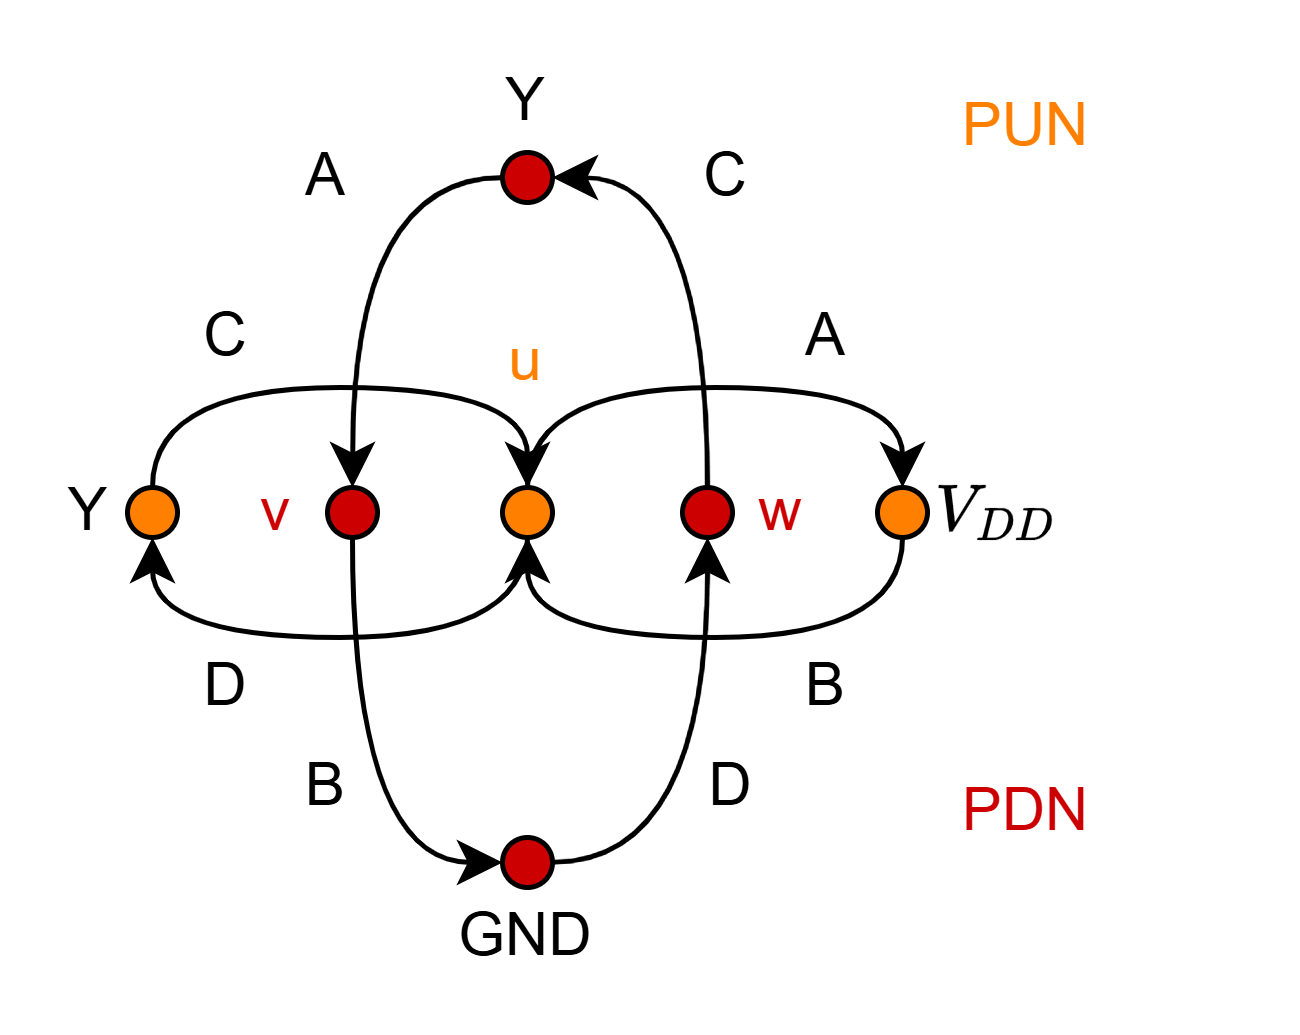
\includegraphics[width=0.45\textwidth]{logic_diagram_problem_2b.png}}}
				\caption{Logic Diagram for Problem 2b Illustrating Euler Path}
				\label{fig::logic_diagram_problem_2b}
			\end{figure}
			
			Finally, with the order of inputs, we can create the stick diagram shown in Figure \ref{fig::stick_diagram_problem_2b}.
			
			\begin{figure}[H]
				\centerline{\fbox{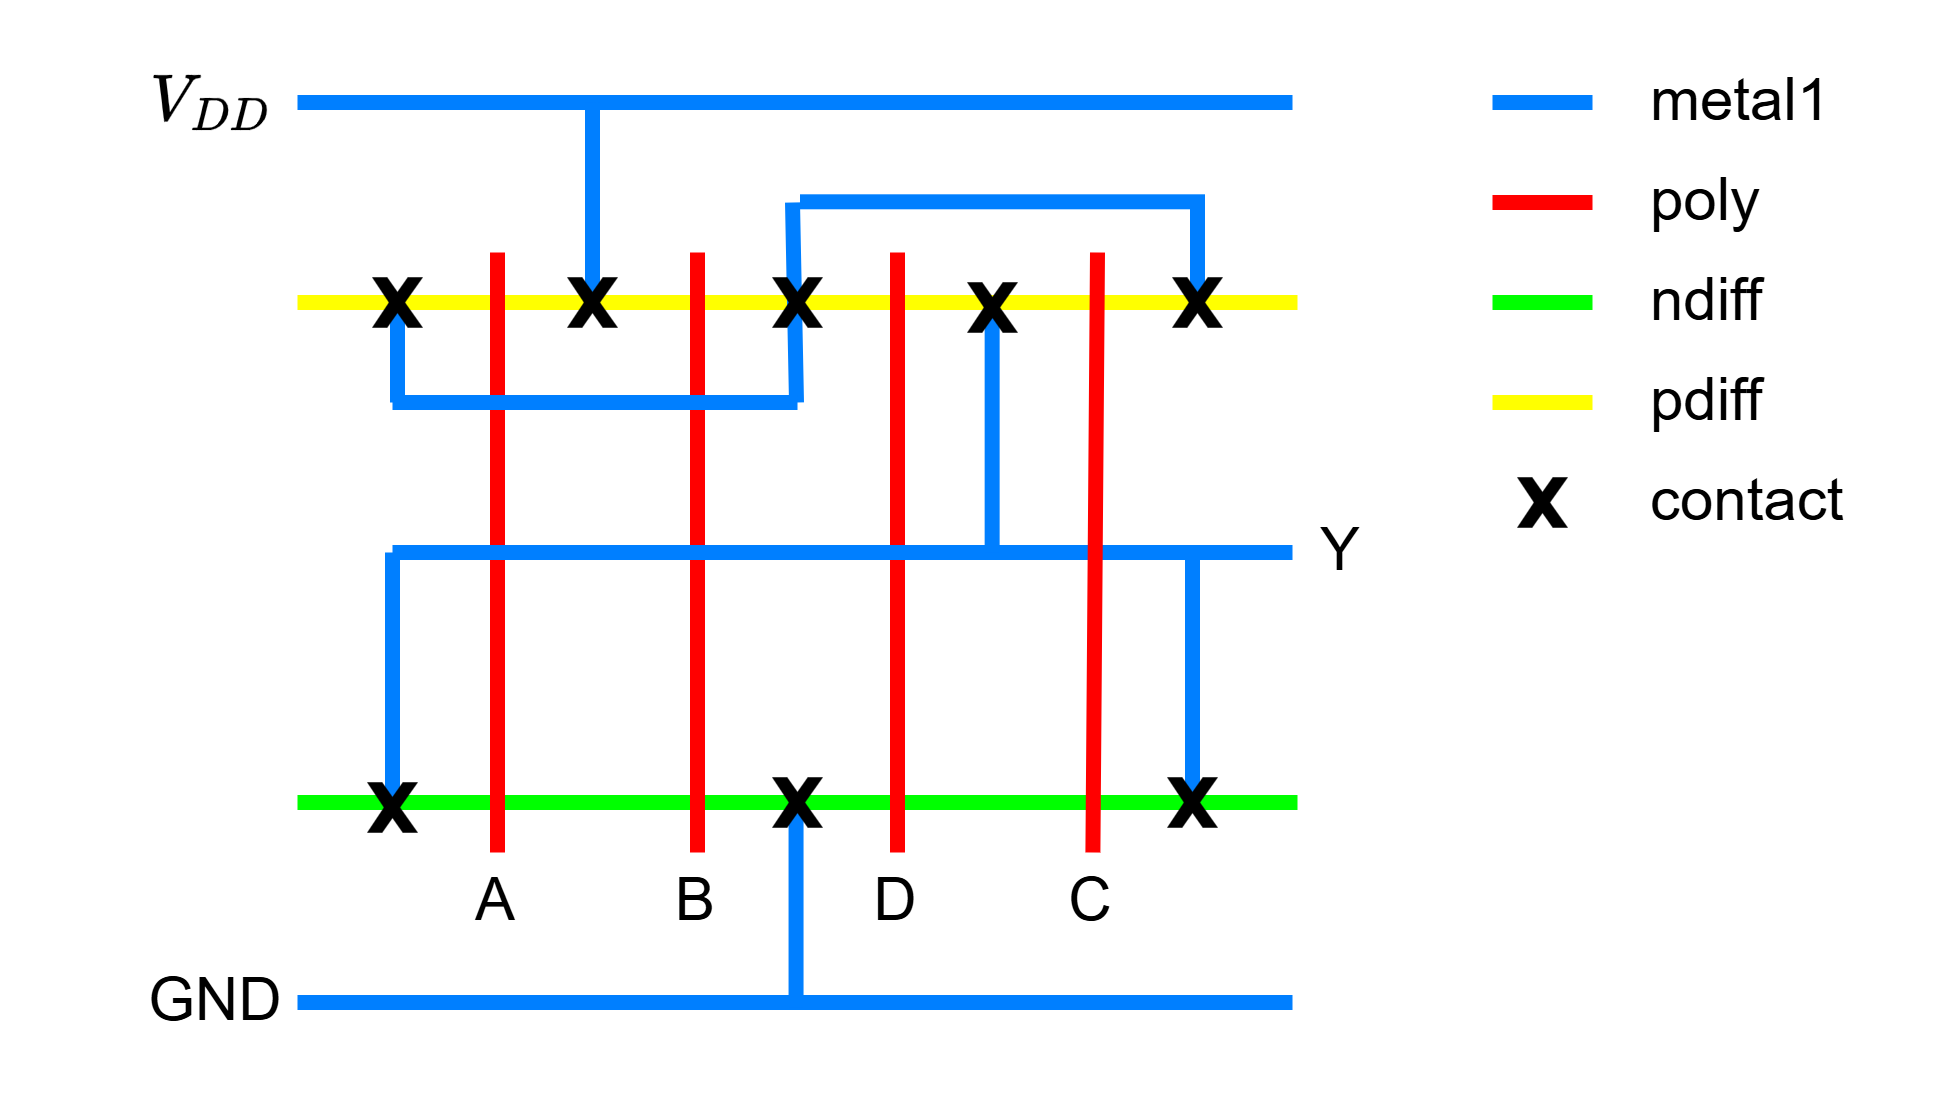
\includegraphics[width=0.5\textwidth]{stick_diagram_problem_2b.png}}}
				\caption{Stick Diagram for Problem 2b}
				\label{fig::stick_diagram_problem_2b}
			\end{figure}
		\end{enumerate}
		
		\item Using the Stick diagrams designed in the previous, question, Calculate the Area Estimation in terms of $\lambda$.
			
		We can estimate the area of the fabricated design by counting wiring tracks. Each wire track has a pitch of $8\lambda$. If we count the number of wires parallel to $V_{DD}$ (including $V_{DD}$), we can estimate the height of the cell. Similarly, we can estimate the width of the cell by counting the number of wires parallel to the polysilicon gates.
		
		For the layout in part a), we can view the circuit as two standard cells (one which produces $\bar{Y}$ and another which inverts it). The first cell is 7 wires tall and 5 wires wide ($56 \lambda \times 40 \lambda$), and the second cell is 4 wires tall and 2 wires wide ($32 \lambda \times 16 \lambda$). However, all our standard cells must have the same height and can only vary in width. Therefore, we must increase the size of the inverter to $56 \lambda \times 16 \lambda$. This results in a total area of $56 \lambda \times 56 \lambda = 3136 \lambda^2$. According to the design rules, the spacing between diffusion regions of adjacent cells must be $4\lambda$ (same as adjacent wires). The size of each cell includes a margin of $2\lambda$ around all edges ($4\lambda$ for each wire and $2\lambda$ on either side of the wire). As a result, our estimate has already taken the spacing between diffusion regions into account.
		
		The area of the layout in part b) is more straightforward to compute. It is 7 wires tall and 5 wires wide, which results in an area of $56 \lambda \times 40 \lambda = 2240\lambda^2$.
		 
		 \item Design and verify a Verilog code for a Ripple Carry Adder with a testbench and simulation waveforms in EDA Playground (using Primis AI) and describe each segment of the code and the testbench. (Please Refer to Installation guide \url{https://docs.primis.ai/rapidgpt-getting-started/}). The submission must include the following:
		 
		 \begin{itemize}
		 	\item Both the Verilog and testbench can either be saved as a word file or as a .v file.
		 	\item The code should be well-structured and commented on to explain each segment using 
Primis AI or your thoughts.
			\item Each section of the Verilog code and testbench should be clearly explained.
			\item Describe how the testbench verifies the correctness of the design. 
			\item The Results window and waveform outputs should be captured and included in the 
submission.
		 \end{itemize}
		 
		 Using Primis AI, I wrote a Verilog ripple carry adder and testbench. These files are included with the submission and are named "ripple\_carry\_adder.v" and "rippler\_carry\_adder\_tb.v" respectively. Within each source file, I added comments to explain how each section of the code works.
		 
		 The ripple carry adder module (\code{ripple\_carry\_adder}) adds inputs \code{a}, \code{b}, and \code{cin}, where \code{a} and \code{b} are input operands that are \code{WIDTH} bits wide and \code{cin} is the input carry bit. The module outputs a \code{sum} that is \code{WIDTH} bits wide and a carry bit, \code{cout}. \code{WIDTH} is a parameter, which can be set by the user when the module is instantiated. This allows the user to instantiate adders of arbitrary width without changing the source code.
		 
		The ripple carry adder is composed of multiple \code{full\_adder} modules - one for each input bit. Each of these full adder modules adds single bits \code{a}, \code{b}, and \code{cin} and outputs single bits \code{sum} and \code{cout}. The carry output (\code{cout}) of each adder module is connected to the carry input (\code{cin}) of the next adder module. The \code{sum} bit is the XOR of \code{a}, \code{b}, and \code{c} bits. The \code{sum} bit is 1 when an odd number of the input its are high (i.e. sum=1 or sum=3). The \code{cout} bit is high when both \code{a} and \code{b} are 1 or when either \code{a} and \code{b} is 1 and \code{c} is 1 (i.e. sum=2 or sum=3). This is the expected behavior for the full adder module.
		
		We use a \code{generate} block to instantiate a variable number of full adder modules. We use a vector of carry bits (\code{carry}) that is \code{WIDTH+1} bits wide to set the input carry bit to each full adder stage and capture the output carry bit of each full adder stage. The first bit in the carry vector is the carry input and each subsequent bit is the output of the previous full adder module. Thus, the \code{WIDTH} bit of the carry vector is the carry bit output of the top-level module. The carry vector combined with the \code{generate} block allow us to easily connect the carry output of one adder module to the input of the next adder module.
		 
		 The ripple carry adder testbench module (\code{ripple\_carry\_adder\_tb}) verifies the behavior of the ripple carry adder. It has no inputs or outputs but instead generates the inputs for the ripple carry adder and compares the ripple carry adder output to the expected output. The testbench contains an instantiation of the ripple carry adder of \code{WIDTH} bits (where \code{WIDTH} defaults to 4):
		 
		 \begin{figure}[H]
		 	\centerline{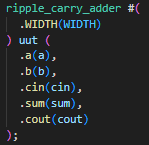
\includegraphics[width=0.25\textwidth]{ripple_carry_adder_inst.png}}
			\caption{Ripple Carry Adder Instantiation}
			\label{fig::ripple_carry_adder_inst}
		 \end{figure}
		 
		 The testbench also generates a clock (\code{clk}) with a 5 ns period. However, this clock is only used in the waveform viewer as a frame of reference for the UUT inputs/outputs. During initialization, the \code{\$dumpfile} and \code{\$dumpvars} command are used to capture signals in the waveform file. After waiting for the system reset (100 ns), the testbench tests the UUT with each combination of \code{a}, \code{b}, and \code{cin} (a total of $2^9=512$ tests). The inputs for each combination are held constant for 10 ns before the adder outputs are compared to reference outputs. For every mismatch, an error message is displayed using \code{\$display} and the number of errors is incremented. The testbench also keeps track of the tests run with an additional counter. After testing all 512 combinations of the inputs, the testbench displays an overall pass/fail result, which simplifies validation. Finally after waiting 100 ns, the simulation terminates. While the simulation is running, the \code{\$monitor} function is also used to monitor changes in the inputs and outputs of the adder.
		  
		 In EDA playground, we run the testbench and verify the behavior of our ripple carry adder. As previously stated, the testbench is validating the output of a 4-bit adder for all 512 combinations of the input. (This is equivalent to validating a 512 entry truth table with 9 inputs and 2 outputs). Using induction, we can infer that the adder should behave accordingly for larger input sizes. Figure \ref{fig::eda_playground_results_window} displays the EDA playground result window. This window captures some of the monitor statements we added in the testbench, but, more importantly, it displays an overall pass, validating the behavior of the design. Figure \ref{fig::eda_playground_waveform} displays the testbench waveform output, which is useful for debugging the design. At the position of the cursor, we can perform a spot check of the results. At this position, a=3, b=10, and cin=1. The measured output is 14, which is the expected value for a+b+cin.
		 
		 \begin{figure}[H]
		 	\centerline{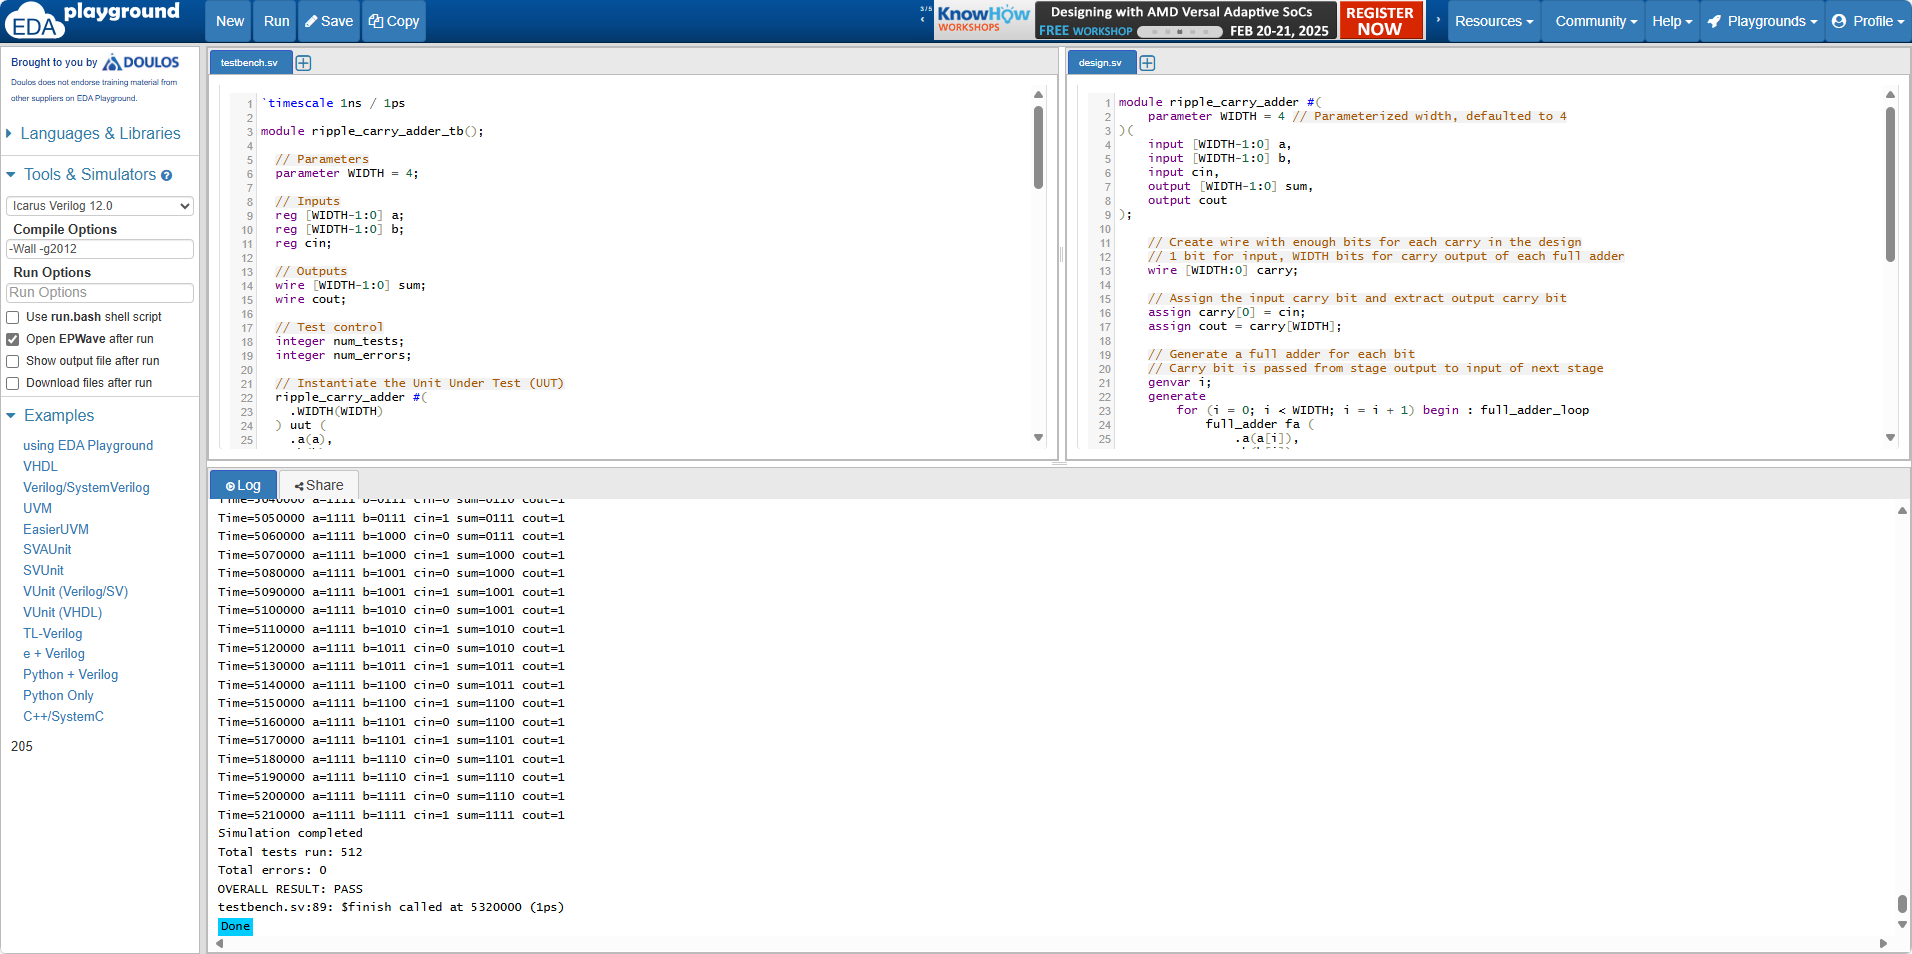
\includegraphics[width=0.9\textwidth]{eda_playground_results_window.png}}
			\caption{EDA Playground Results Window}
			\label{fig::eda_playground_results_window}
		 \end{figure}
		 
		 \begin{figure}[H]
		 	\centerline{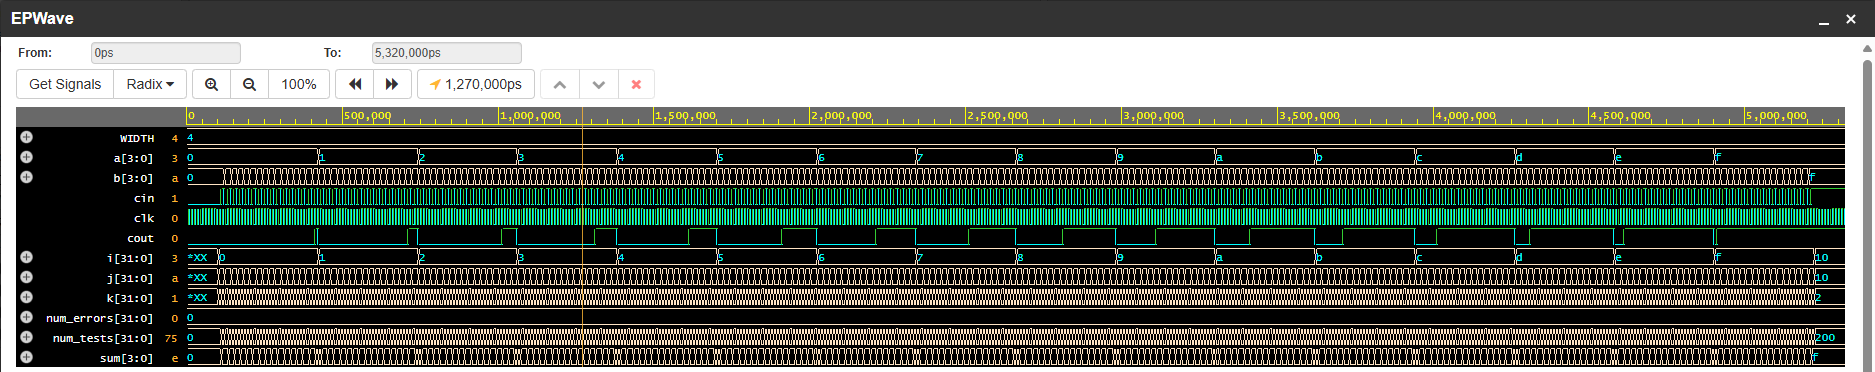
\includegraphics[width=0.9\textwidth]{eda_playground_waveform.png}}
			\caption{EDA Playground Waveform Output}
			\label{fig::eda_playground_waveform}
		 \end{figure}
		 
		 \iffalse
		 \includegraphics[width=0.9\textwidth]{ripple_carry_adder_ai_prompt1.png}
		 
		 \includegraphics[width=0.9\textwidth]{ripple_carry_adder_ai_prompt2.png}
		 
		 \includegraphics[width=0.9\textwidth]{ripple_carry_adder_ai_prompt3.png}
		 
		 \includegraphics[width=0.9\textwidth]{ripple_carry_adder_ai_prompt4.png}
		 
		 \includegraphics[width=0.9\textwidth]{ripple_carry_adder_ai_prompt5.png}
		 
		 \includegraphics[width=0.9\textwidth]{ripple_carry_adder_ai_prompt6.png}
		 %\begin{figure}[H]
		%	\centerline{\includegraphics[width=0.9\textwidth]{ripple_carry_adder_ai_prompt1.png}}
			% \caption{Stick Diagram for Problem 2b}
		%	\label{fig::ripple_carry_adder_ai_prompt1}
		%\end{figure}
			
		 The verilog code and testbench generated using Primis AI are attached in Appendix \ref{appendix::ripple_carry_adder} and Appendix \ref{appendix::testbench} respectively. 
		 \fi
	\end{enumerate}
	
	\iffalse
	\pagebreak
	\appendix
	\section{Verilog Ripple Carry Adder Written with Primis AI}
	\label{appendix::ripple_carry_adder}
	\lstset{style={verilog-style}}
	\lstinputlisting{ripple_carry_adder.v}
	
	\pagebreak
	\section{Verilog Testbench Written with Primis AI}
	\label{appendix::testbench}
	\lstset{style={verilog-style},showstringspaces=false}
	\lstinputlisting{ripple_carry_adder_tb.v}
	\fi
\end{document}